\subsection{Forward Tagger (FT)}


\subsubsection{Geometry}

The FT consists of three subsystems:

\begin{itemize}
	\item a tracker (FT-TRK), composed by 4 micromegas layers;
	\item a hodoscope (FT-HODO), with eight sectors, each containing two layers of scintillators;
 	\item a calorimeter (FT-CAL) containing an array of 332 crystals.
\end{itemize}

The three subsystems are implemented in GEMC using the native perl API script, except for the inner shield (see Section \ref{sec:beamline}),
which comes from the CAD engineering model.
The FT geometry is shown in \F{ftGeometry}.

\subsubsection{Digitization}

\begin{figure}
	\centering
	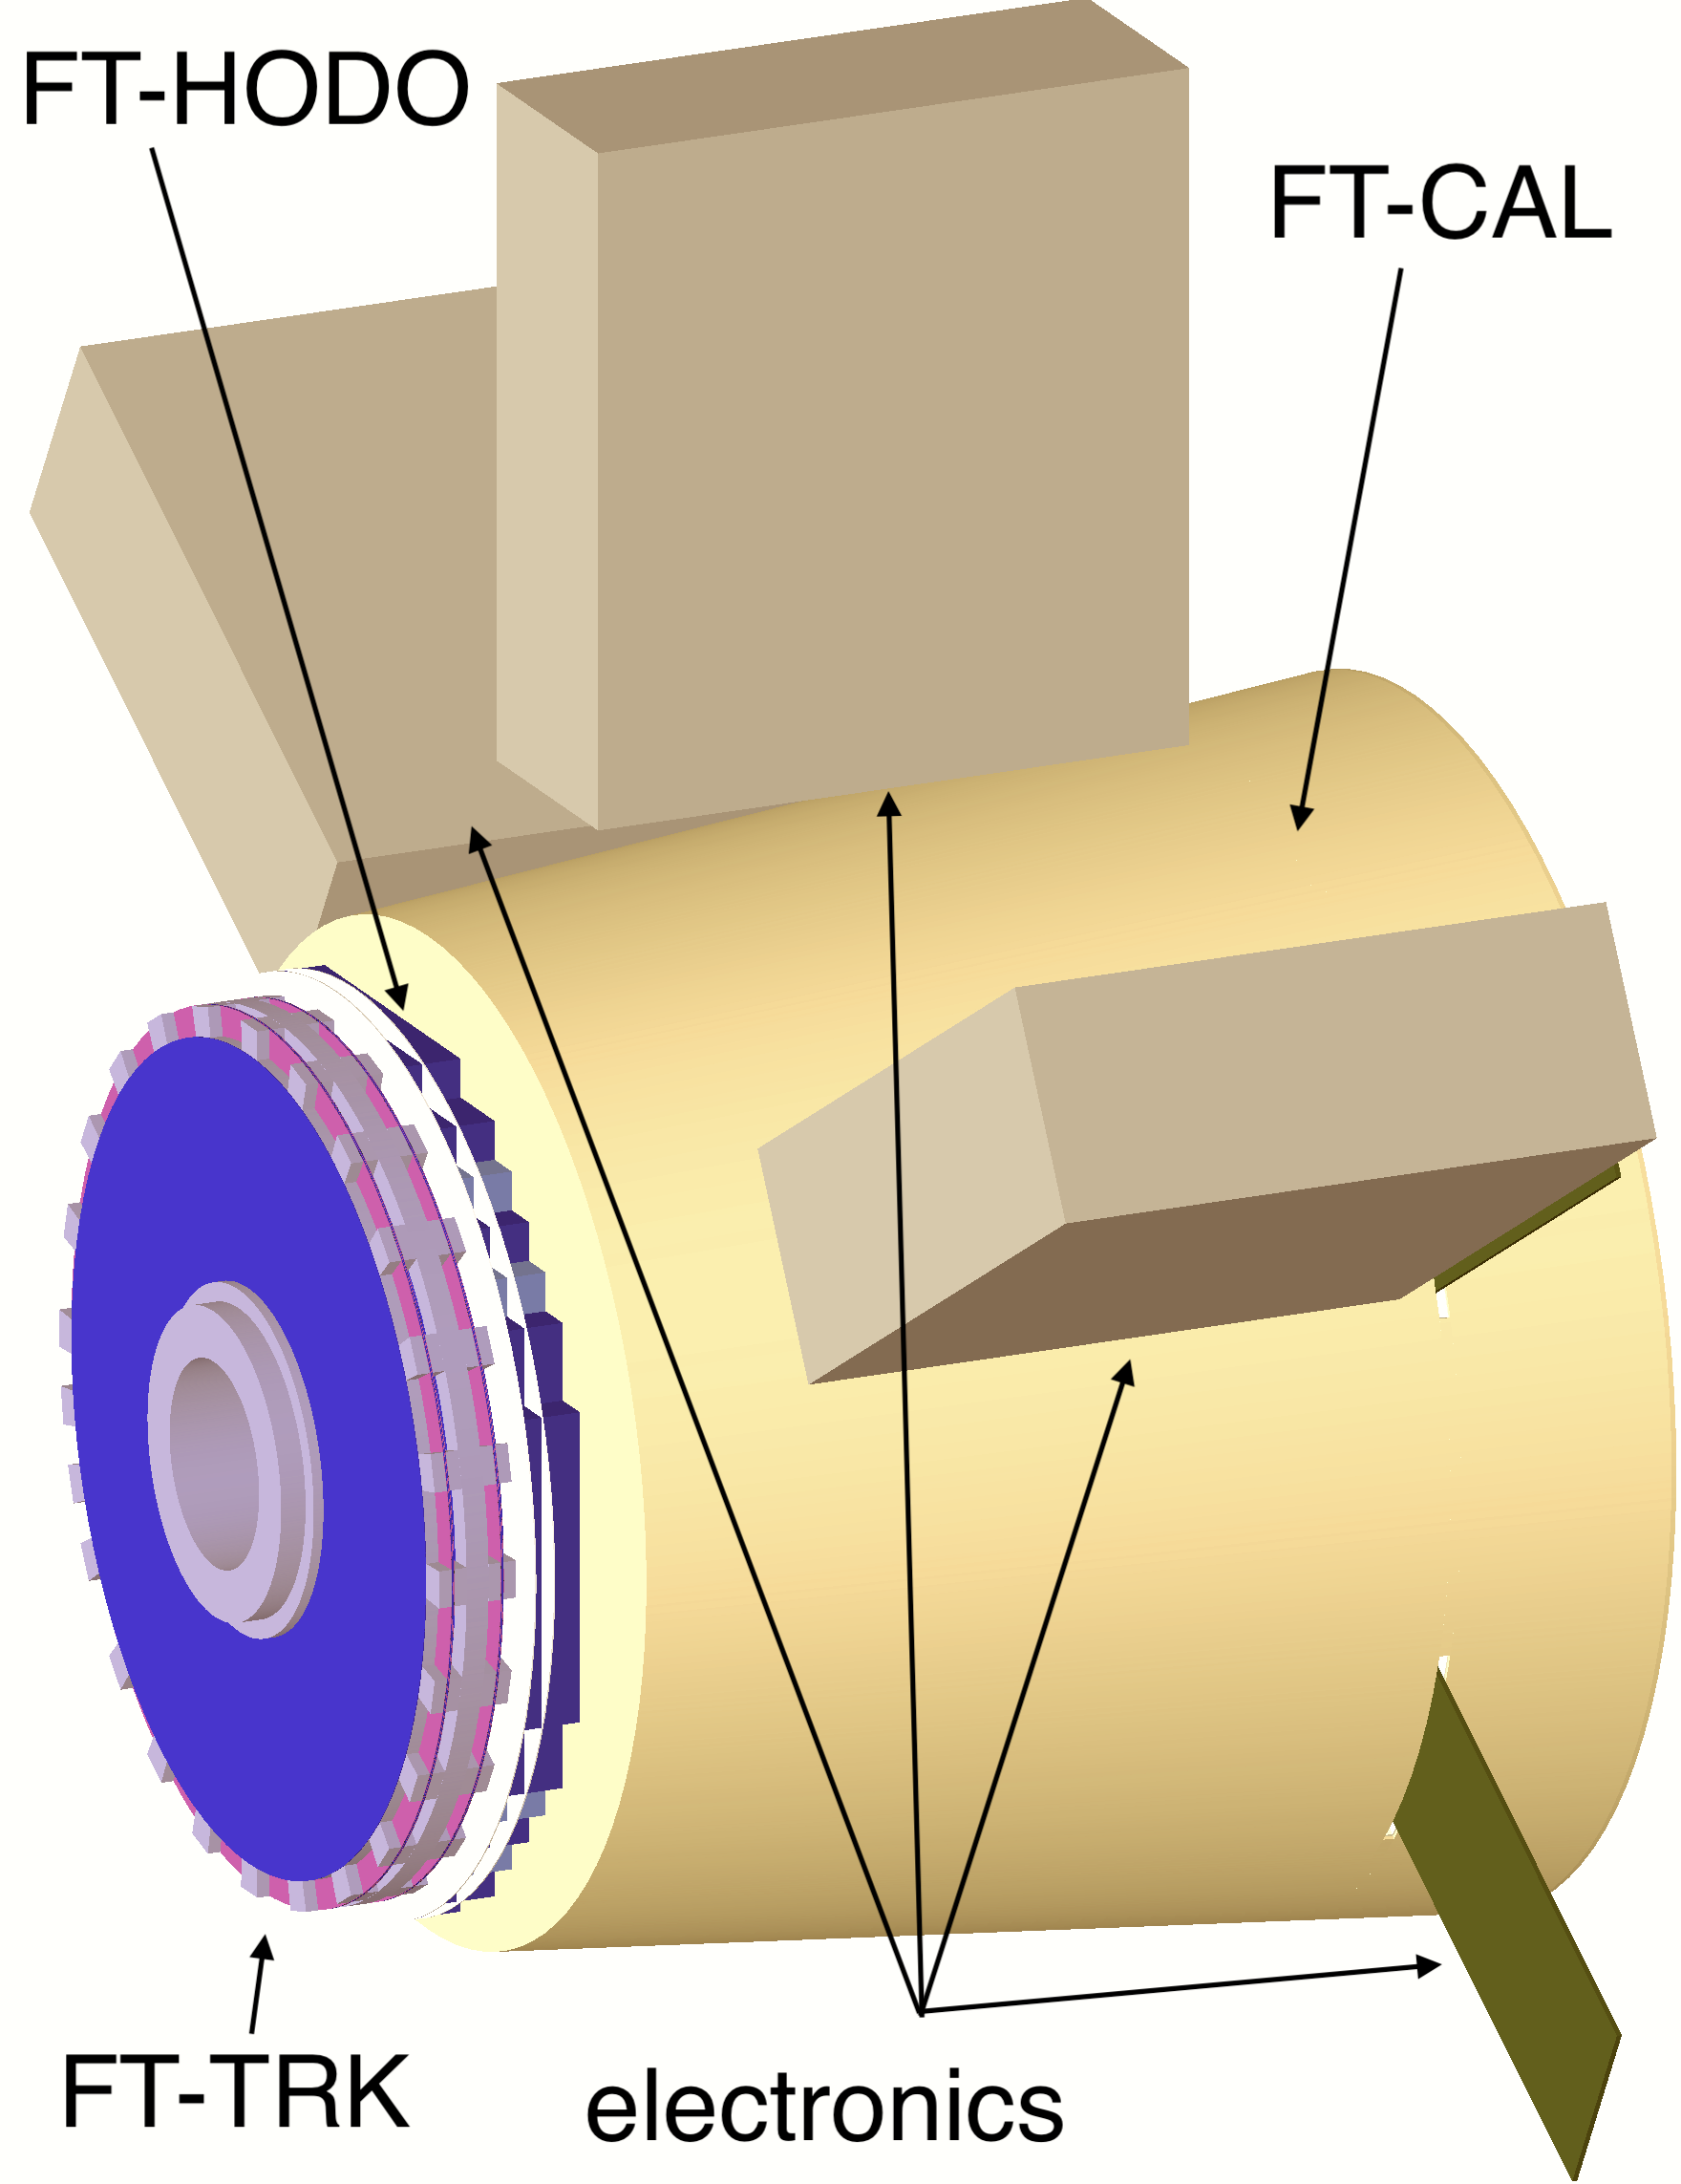
\includegraphics[width=0.99\columnwidth,keepaspectratio]{img/ftGeometry.png}
	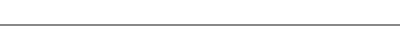
\includegraphics[width=0.99\columnwidth,keepaspectratio]{img/blank.png}
	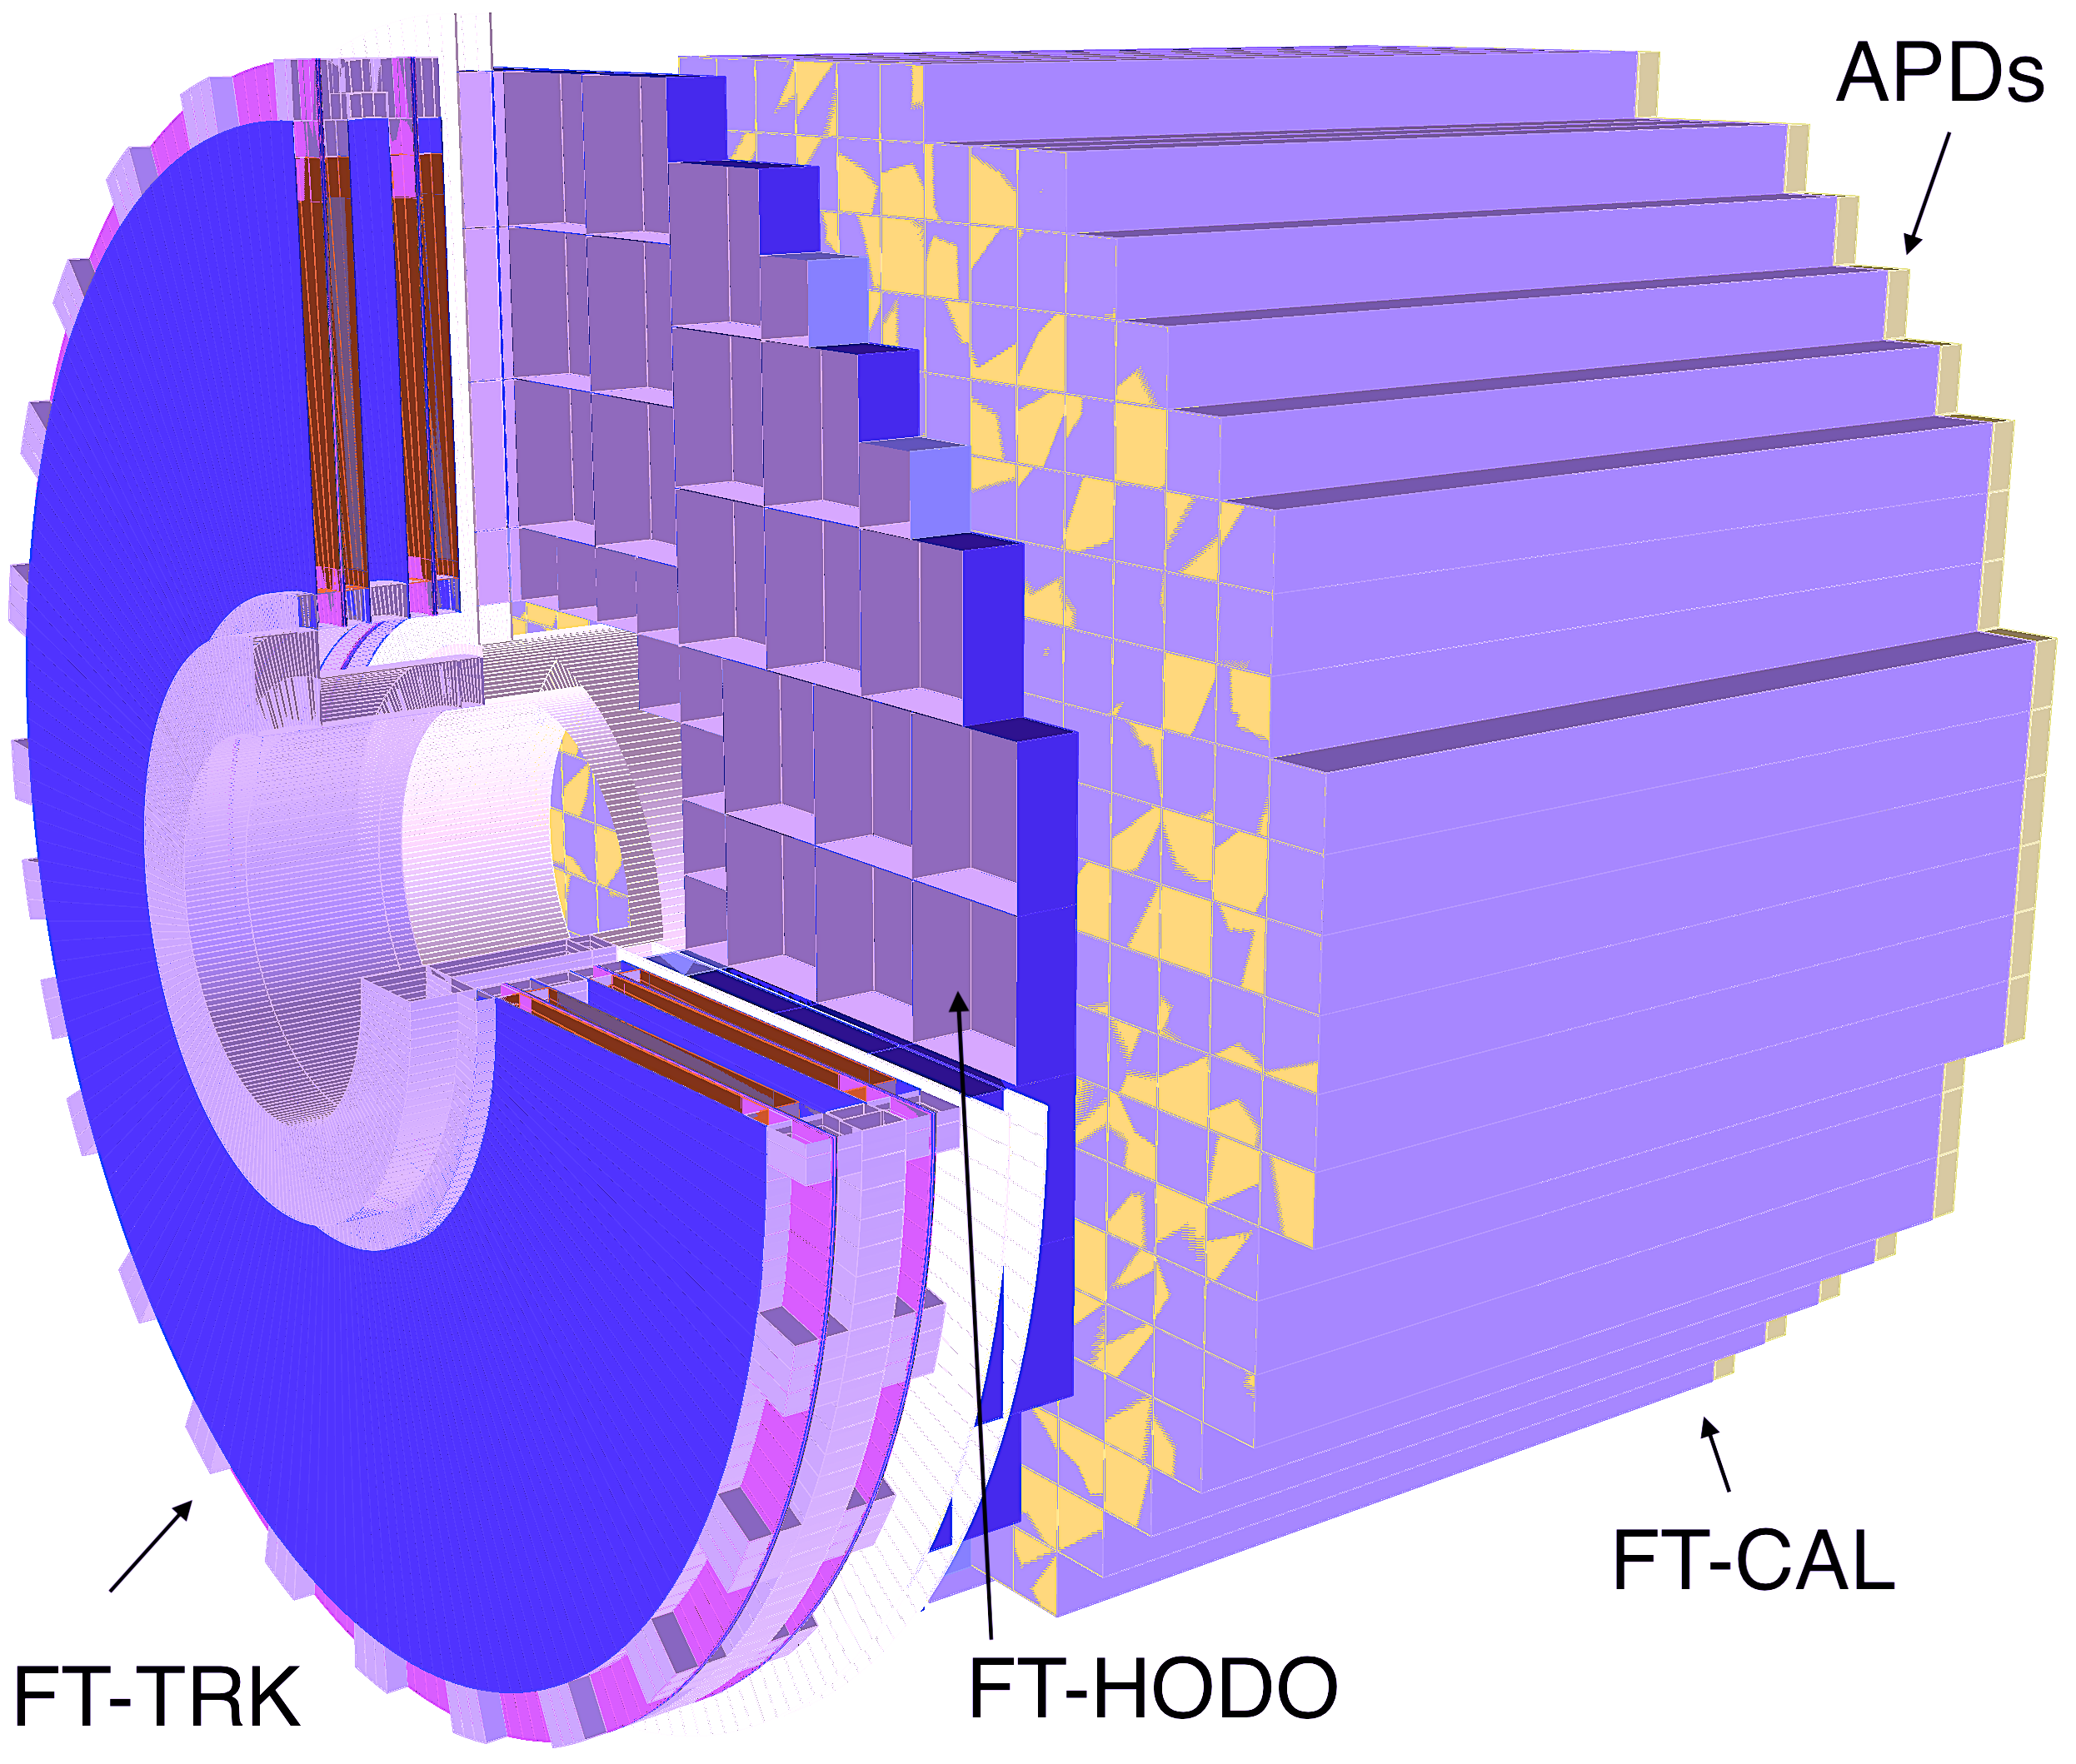
\includegraphics[width=0.99\columnwidth,keepaspectratio]{img/ftDetails.png}
	\caption{Top: the FT detector implementation in GEMC. The boxes surrounding FT-CAL contain the electronics.
			 Bottom: details of the implementation of the three subsystems. As seen by the beam (incident from the left):
             the disks form the FT-TRK; the FT-HODO scintillators just behind the tracker;
			 and the FT-CAL crystals. }
	\label{fig:ftGeometry}
\end{figure}

The FT-TRK digitization provides the ADC value calculated using the total energy deposited (after hit sharing).
There is no timing information in the FT-TRK output.

For FT-CAL hits, the energy deposited is converted first to the charge produced at the end of the electronics chain composed
by an avalanche photo-diode (APD) and pre-amplifier, and then to an ADC.
The first conversion is based on the measured charge for cosmic rays that deposit a known energy in the crystals,
while the second conversion is based on the FADC conversion factor. A smearing on the final ADC values is added,
accounting for the Poisson distribution of photo-electrons produced by the photo-sensor, the Gaussian noise of the
photo-sensor, and of the pre-amplifier. All parameters, the number of photo-electrons per MeV of energy deposited,
the RMS width of the APD noise, and of the pre-amplifier input noise, have been tuned to the experimental data.

The same approach is adopted to process FT-HODO hits. The output is read by silicon photo-multipliers
(included in the simulation) in which the deposited energy is first converted to charge and
then to ADC.
The smearing in this case accounts only for the Poisson distribution of the measured number of photo-electrons,
which dominates over other sources because of the relatively small number of photo-electrons per MeV of energy deposition.

The TDC of FT-CAL hits is computed from the time of the energy deposition, accounting for the speed of the scintillation light in
the crystal and the distance to the photo-sensor, assuming a known time-to-TDC conversion factor. A Gaussian smearing on the
resulting TDC is added based on a fixed RMS resolution derived from the experimental measurements.

Similarly, the TDC of FT-HODO hits is derived from the time of a given energy deposition, adding a fixed offset before the
conversion from time to TDC and a Gaussian smearing. As in previous cases, all relevant parameters have been tuned to the
observed detector response.
The digitized output bank variables are summarized in Table \ref{tab:ftBank}.

\begin{table}[h]
	\begin{center}
		\begin{tabular}{| c | c | c |}
			\hline \hline
			Variable            & Description      \\
			\hline
		                         & Tracker         \\
			\hline
                          layer  &      tracker layer \\
                      component  &  strip number      \\
                            ADC  &        ADC         \\
			\hline
		                         & Hodoscope          \\
			\hline
						 sector  &     hodoscope sector  \\
                          layer  &      hodoscope layer  \\
                      component  &  tile number    \\
                            ADC  &        ADC      \\
                            TDC  &        TDC      \\
			\hline
								 & Calorimeter     \\
			\hline
					  component  &  crystal number \\
							ADC  &        ADC      \\
							TDC  &        TDC      \\
			\hline \hline
		\end{tabular}
	\end{center}
	\caption{The digitized FT banks for the tracker, hodoscope, and calorimeter}\label{tab:ftBank}
\end{table}

\noindent The time window  of the Tracker is set to to 132 ns: all Geant4 steps within the same strip and time window are collected in one hit.
The time window of the hodoscope and calorimeters are set to 400 ns: all Geant4 steps within the same paddles and time window
will be collected on one hit in each system.
